\documentclass[12pt]{article}
\usepackage[utf8]{inputenc}
\usepackage{geometry}
\usepackage{amsfonts}
\usepackage{hyperref}
\usepackage{enumitem}
\usepackage{graphicx}
\usepackage{tabularx}
\usepackage{multirow}
\usepackage{amsmath}
\usepackage{xcolor}
\usepackage{array}
\usepackage{tikz}


\title{
    \textbf{CSE343: Machine Learning} \\ \vspace*{-5pt}
    \textbf{\large{Assignment-2}}
}

\author{\href{mailto:divyajeet21529@iiitd.ac.in}{Divyajeet Singh (2021529)}}
\date{\today}

\geometry{a4paper, left=20mm, right=20mm, top=20mm, bottom=20mm}


\begin{document}
    \maketitle

    \section{Section A (Theoretical)}
    \subsection*{Solution 1}

    \subsubsection*{(a) (1 mark)}
    \subsubsection*{Solution}
    A random forest consists of many trees. Correlation refers to the similarity
    between trees - similar trees capture similar patterns in the data. Diversity,
    on the other hand, refers to the difference in the trees. With a large number of
    trees, we get a balanced prediction from the forest, which is able to capture
    most of the patterns in the data and make better predictions. \\
    However, if the trees are too diverse and have very little correlation,
    this could mean that the bigger patterns are not being effectively covered. This
    can reduce the performance of the trees. So, it is important to maintain some
    diveristy among a forest of correlated trees.

    \subsubsection*{(b) (1 mark)}
    \subsubsection*{Solution}
    Naïve Bayes works by predicting the class labels that maximize the posterior
    probability using Bayes' Theorem, assuming that the features are independent of
    each other. \\
    With the curse of dimensionality (excessive number of features), the dataset in
    consideration can be very sparse. Naïve Bayes performs poorly on sparse datasets,
    since it predicts a 0 probability for a feature that it has not seen before.
    Moreover, it assumes that all feautres are weighed equally, which can cause
    issues with its performance with a large number of features. \\
    To solve this problem, one can use dimensionality reduction techniques like
    Principal Component Analysis (PCA) or Linear Discriminant Analysis (LDA),
    and smoothing techniques like Laplace smoothing to prevent 0 probabilities.

    \subsubsection*{(c) (1 mark)}
    \subsubsection*{Solution}
    When Naïve Bayes encounters a value of an attribute that it has not seen before,
    it assigns a 0 probability to it. This clearly affects the performance of the
    model adversely as it can return a probability of 0 for inputs having large
    probabilities for other attributes, thereby increasing its variance. For
    example, consider the dataset in Table \ref{tab:dataset}.
    \begin{table}[htbp]
        \centering
        \begin{tabular}{cc|c}
            \textsc{Weather} & \textsc{Humidity} & \textsc{Will-play} \\
            \hline
            \texttt{Hot} & \texttt{High} & \textbf{0} \\
            \texttt{Hot} & \texttt{Low} & \textbf{0} \\
            \texttt{Cool} & \texttt{High} & \textbf{1} \\
            \texttt{Cool} & \texttt{Low} & \textbf{1}
        \end{tabular}
        \caption{A sample dataset for Naïve Bayes}
        \label{tab:dataset}
    \end{table}
    \vspace*{0pt} \\
    It is obvious that the target variable depends solely on the \textsc{Weather}.
    However, the Naïve Bayes model would predict the class \textbf{0} for an
    input vector \texttt{[Cool, Mid]} since it has not seen the \textsc{Humidity}
    attribute before.
    This effect can be avoided by using smoothing techniques like Laplace smoothing
    and m-estimate, which add a small positive value to the probability of each
    attribute, even for the features that are not present in the datset. This
    prevents an unwanted \textbf{0} as the probability of a class.

    \subsubsection*{(d) (1 mark)}
    \subsubsection*{Solution}
    \textbf{Yes}, the cardinality of the attributes affects the splitting of
    a tree node when using Information Gain. This means that for two feaures
    that produce equally good splits, the one with the higher cardinality will
    be chosen. \\
    An alternative way is to use Gain Ratio instead of Information Gain to choose
    splits. This is a normalized version of Information Gain, which takes into
    account the cardinality of the attributes. This ensures that the attribute
    with the higher cardinality is not favoured over the other.
    $$\textsc{Gain-ratio} = \frac{\textsc{Info-gain}}{\textsc{Split-Info}}$$
    where
    $$\textsc{Split-info} = -\sum_{i=1}^{n} \frac{N(t_{i})}{N_{t}} \log_{2}{\frac{N(t_{i})}{N_{t}}}$$
    For example, let's say a dataset consists of 90 unique ages and 10000
    unique Customer IDs. Then, the attribute \textsc{Customer ID} will be
    favoured over \textsc{Age} when using Information Gain, even though
    \textsc{Customer ID} cannot be a good indicator of the target variable.

    \subsection*{Solution 2}
    \subsubsection*{(a) (1 mark)}
    \subsubsection*{Solution}
    Let the random variable $R$ represent "Can borrow racket?", $F$ reprsent "$>$ 7 friends?", and $W$ represent "Weather".
    Then, there are four possible outcomes in the given problem. These are listed with their conditional probability expressions in Table \ref{tab:prob}. The decision
    tree is given in Figure \ref{fig:tree}.
    \begin{table}[htbp]
        \centering
        \begin{tabular}{l|l}
            \textsc{Outcome} ($Y$) & \textsc{Conditional Probability} \\
            \hline
            \texttt{TT (T)} & $\mathbb{P}[Y = \texttt{T} \ | \ R = \texttt{Yes}] * \mathbb{P}[R = \texttt{Yes} \ | \ W = \texttt{Rain}] * \mathbb{P}[W = \texttt{Rain}]$ \\
            \texttt{Pool (P)} & $\mathbb{P}[Y = \texttt{P} \ | \ R = \texttt{No}] * \mathbb{P}[R = \texttt{No} \ | \ W = \texttt{Rain}] * \mathbb{P}[W = \texttt{Rain}]$ \\
            \texttt{Football (F)} & $\mathbb{P}[Y = \texttt{F} \ | \ F = \texttt{Yes}] * \mathbb{P}[F = \texttt{Yes} \ | \ W = \texttt{Clear}] * \mathbb{P}[W = \texttt{Clear}]$ \\
            \texttt{Badminton (B)} & $\mathbb{P}[Y = \texttt{B} \ | \ F = \texttt{No}] * \mathbb{P}[F = \texttt{No} \ | \ W = \texttt{Clear}] * \mathbb{P}[W = \texttt{Clear}]$
        \end{tabular}
        \caption{Conditional Probabilities for the given problem}
        \label{tab:prob}
    \end{table}
    \vspace*{0pt} \\
    \begin{center}
        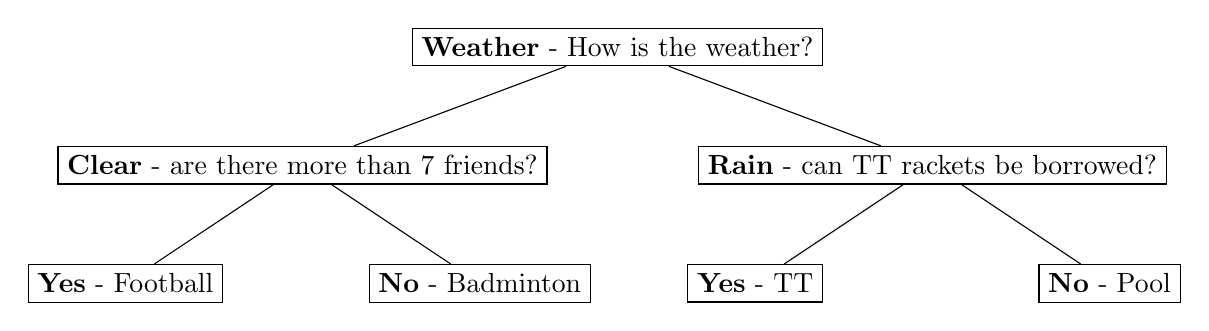
\begin{tikzpicture}
            [level/.style={sibling distance=45mm/#1},
            every node/.style={draw, rectangle, align=center},
            level 1/.style={sibling distance=80mm},
            level 2/.style={sibling distance=45mm}]

            \node {\textbf{Weather} - How is the weather?}
            child {
                node {\textbf{Clear} - are there more than 7 friends?}
                child {node {\textbf{Yes} - Football}}
                child {node {\textbf{No} - Badminton}}
            }
            child {
                node {\textbf{Rain} - can TT rackets be borrowed?}
                child {node {\textbf{Yes} - TT}}
                child {node {\textbf{No} - Pool}}
            };
            \label{fig:tree}
        \end{tikzpicture}
    \end{center}

    \subsubsection*{(b) (1 mark)}
    \subsubsection*{Solution}
    Let us define two random variables $P$ and $T$ to represent the prediction
    of the app and the truth respectively. Both of them can take values from
    the set $\{ \texttt{R}, \texttt{C} \}$, where \texttt{R} and \texttt{C}
    represent \texttt{Rain} and \texttt{Clear} respectively. \\
    We are given that the app correctly predicts rainy days with an 80\% accuracy
    and clear days with a 90\% accuracy. This means that
    \begin{align}
        \mathbb{P}[P = \texttt{R} \ | \ T = \texttt{R}] &= 0.8 \implies \mathbb{P}[P = \texttt{C} \ | \ T = \texttt{R}] = 0.2 \\
        \mathbb{P}[P = \texttt{C} \ | \ T = \texttt{C}] &= 0.9 \implies \mathbb{P}[P = \texttt{R} \ | \ T = \texttt{C}] = 0.1
    \end{align}
    We are also given that the app predicts rain on 30\% of the days. This means
    \begin{align}
        \label{eq:prob}
        \mathbb{P}[P = \texttt{R}] &= 0.3 \implies \mathbb{P}[P = \texttt{C}] = 0.7
    \end{align}
    Let us find the probability that it rains on a day when the app predicts rain.
    \begin{align}
        \mathbb{P}[T = \texttt{R} \ | \ P = \texttt{R}] &= \frac{\mathbb{P}[P = \texttt{R} \ | \ T = \texttt{R}] * \mathbb{P}[T = \texttt{R}]}{\mathbb{P}[P = \texttt{R}]} \\
        \label{eq:prob2}
        &= \frac{0.8 * \mathbb{P}[T = \texttt{R}]}{0.3}
    \end{align}
    To find the probability that it rains on a day, we use the law of total probability
    on Equation \eqref{eq:prob}. Note that $\{ T = \texttt{R} \}$ and $\{ T = \texttt{C} \}$ are
    complementary events.
    \begin{align}
        \mathbb{P}[P = \texttt{R}] &= \mathbb{P}[P = \texttt{R} \ | \ T = \texttt{R}] \ \mathbb{P}[T = \texttt{R}] + \mathbb{P}[P = \texttt{R} \ | \ T = \texttt{C}] \ \mathbb{P}[T = \texttt{C}] \\
        0.3 &= 0.8 * \mathbb{P}[T = \texttt{R}] + 0.1 * (1 - \mathbb{P}[T = \texttt{R}]) \\
        0.3 &= 0.1 + 0.7 * \mathbb{P}[T = \texttt{R}] \\
        \implies \mathbb{P}[T = \texttt{R}] &= \frac{0.2}{0.7} \\
    \end{align}
    Substituting this value in Equation \eqref{eq:prob2}, we get
    \begin{align}
        \mathbb{P}[T = \texttt{R} \ | \ P = \texttt{R}] &= \frac{0.8 * \frac{0.2}{0.7}}{0.3} = \frac{16}{21} \approx 0.7619
    \end{align}
    Therefore, the required probability is approximately 0.762.

    \subsubsection*{(c) (1.5 marks)}
    \subsubsection*{Solution}
    In the updated question, Rahul decides whether to play or go to the gym based on
    his mood. So, the updated decision tree is given in Figure \ref{fig:tree2}.
    \begin{center}
        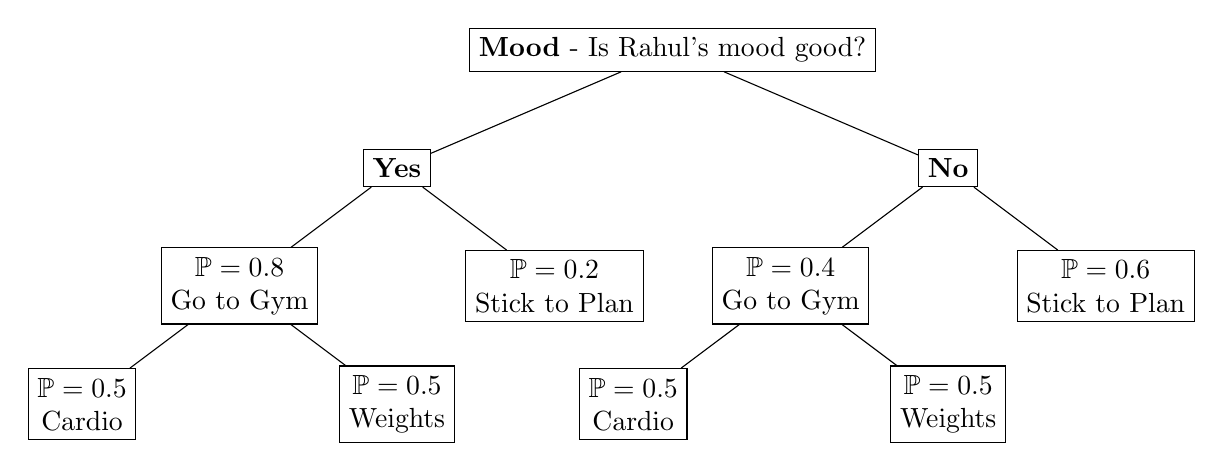
\begin{tikzpicture}
            [level/.style={sibling distance=45mm/#1},
            every node/.style={draw, rectangle, align=center},
            level 1/.style={sibling distance=70mm},
            level 2/.style={sibling distance=40mm},
            level 3/.style={sibling distance=40mm}]

            \node {\textbf{Mood} - Is Rahul's mood good?}
            child {
                node {\textbf{Yes}}
                child {
                    node {$\mathbb{P} = 0.8$ \\ Go to Gym}
                    child {node {$\mathbb{P} = 0.5$ \\ Cardio}}
                    child {node {$\mathbb{P} = 0.5$ \\ Weights}}
                }
                child {node {$\mathbb{P} = 0.2$ \\ Stick to Plan}}
            }
            child {
                node {\textbf{No}}
                child {
                    node {$\mathbb{P} = 0.4$ \\ Go to Gym}
                    child {node {$\mathbb{P} = 0.5$ \\ Cardio}}
                    child {node {$\mathbb{P} = 0.5$ \\ Weights}}
                }
                child {node {$\mathbb{P} = 0.6$ \\ Stick to Plan}}
            };
            \label{fig:tree2}
        \end{tikzpicture}
    \end{center}
    Let $M$ represent Rahul's mood, which can take values from $\{ \texttt{G}, \texttt{B} \}$, where \texttt{G} and \texttt{B} represent \texttt{Good} and \texttt{Bad} respectively.
    Let $A$ represent the chosen activity, which can take values from $\{ \texttt{Gym}, \texttt{Stick-to-plan} \}$.
    Then, the list of outcomes along with the expressions for their conditional probabilities
    is given below.
    \begin{enumerate}
        \item Stick to Plan\footnote{
            This option is essentially the tree given in Figure \ref{fig:tree}, starting
            from the root. We calculate the probability of this outcome as a whole - as will
            be seen next, this will not change the answer since the probability of this tree
            as a whole will be less than the most likely activity.
        } (\texttt{S}) \begin{align*}
            &\mathbb{P}[Y = \texttt{S} \ | \ M = \texttt{G}] * \mathbb{P}[M = \texttt{G}] + \mathbb{P}[Y = \texttt{S} \ | \ M = \texttt{B}] * \mathbb{P}[M = \texttt{B}] \\
            &= 0.2 * \mathbb{P}[M = \texttt{G}] + 0.6 * \mathbb{P}[M = \texttt{B}]
        \end{align*}

        \item Do Cardiological Exercises (\texttt{C}) \begin{align*}
            &\mathbb{P}[Y = \texttt{C} \ | \ A = \texttt{Gym}] * \mathbb{P}[A = \texttt{Gym} \ | \ M = \texttt{G}] * \mathbb{P}[M = \texttt{G}] + \\
            &\mathbb{P}[Y = \texttt{C} \ | \ A = \texttt{Gym}] * \mathbb{P}[A = \texttt{Gym} \ | \ M = \texttt{B}] * \mathbb{P}[M = \texttt{B}] \\
            &= 0.5 * 0.8 * \mathbb{P}[M = \texttt{G}] + 0.5 * 0.4 * \mathbb{P}[M = \texttt{B}]
        \end{align*}

        \item Do Weight Training (\texttt{W}) \begin{align*}
            &\mathbb{P}[Y = \texttt{W} \ | \ A = \texttt{Gym}] * \mathbb{P}[A = \texttt{Gym} \ | \ M = \texttt{G}] * \mathbb{P}[M = \texttt{G}] + \\
            &\mathbb{P}[Y = \texttt{W} \ | \ A = \texttt{Gym}] * \mathbb{P}[A = \texttt{Gym} \ | \ M = \texttt{B}] * \mathbb{P}[M = \texttt{B}] \\
            &= 0.5 * 0.8 * \mathbb{P}[M = \texttt{G}] + 0.5 * 0.4 * \mathbb{P}[M = \texttt{B}]
        \end{align*}
    \end{enumerate}

    \subsubsection*{(d) (1.5 marks)}
    \subsubsection*{Solution}
    We are given the following (here, $F$ repsents the number of hours of sleep Rahul got the previous night)
    \begin{align}
        \mathbb{P}[M = \texttt{G}] &= 0.6 &\quad \mathbb{P}[M = \texttt{B}] &= 0.4 \\
        \mathbb{P}[F = 7 \ | \ M = \texttt{G}] &= 0.7 &\quad \mathbb{P}[F = 7 \ | \ M = \texttt{B}] &= 0.45
    \end{align}
    First, we find out the probability that Rahul is in a good mood, given he slept for 7 hours
    the previous night.
    \begin{align}
        \mathbb{P}[M = \texttt{G} \ | \ F = 7] &= \frac{\mathbb{P}[F = 7 \ | \ M = \texttt{G}] * \mathbb{P}[M = \texttt{G}]}{\mathbb{P}[F = 7 \ | \ M = \texttt{G}] * \mathbb{P}[M = \texttt{G}] + \mathbb{P}[F = 7 \ | \ M = \texttt{B}] * \mathbb{P}[M = \texttt{B}]} \\
        &= \frac{0.7 * 0.6}{0.7 * 0.6 + 0.45 * 0.4} = \frac{42}{60} = 0.7
    \end{align}
    Now, we simply substitute the value of $\mathbb{P}[M = \texttt{G} \ | \ F = 7]$ in the conditional
    probabilities of the outcomes to get the required probabilities. Note that Rahul's mood being good
    or bad are complementary events.
    \begin{enumerate}
        \item Stick to Plan: $\mathbb{P}[Y = \texttt{S}] = 0.2 * 0.7 + 0.6 * 0.3 = 0.32$
        \item Do Cardiological Exercises: $\mathbb{P}[Y = \texttt{C}] = 0.5 * 0.8 * 0.7 + 0.5 * 0.4 * 0.3 = 0.34$
        \item Do Weight Training: $\mathbb{P}[Y = \texttt{W}] = 0.5 * 0.8 * 0.7 + 0.5 * 0.4 * 0.3 = 0.34$
    \end{enumerate}
    Since the probability of sticking to the original plan of playing games is already lower than the
    probabilities of the other two outcomes, the answer does not change. Since the "Stick to Plan" option
    is further divided in the decision tree in Figure \ref{fig:tree}, the probability of the outcomes
    of the four games are naturally smaller than the probability of the "Stick to Plan" option as a whole.
    This means that they cannot be the most likely outcome. \\
    Hence, the most likely outcome is to do either cardiological exercises or weight training.

    \section{Section B (Library Implementation)}
    This section required us to use the Decision Tree and Random Forest Classifiers in Python to predict
    the presence of heart diseases using the \href{https://archive.ics.uci.edu/dataset/45/heart+disease}{\color{blue}\underline{UCI Heart Disease Dataset}}.
    The \texttt{scikit-learn} package was used for this problem. The solution can be found in the
    \texttt{main.ipynb} notebook.

    \subsection*{Best Criterion for Splitting in Decision Trees}
    An exploratory data analysis was performed on the dataset. For the given dataset, I averaged the performance of
    D-Trees trained using both criterions over more than 10,000 runs.
    It was clear that (both for the binary and multiclass classification), the Gini Impurirt criterion performed better than the Entropy criterion.
    The results are shown in Table \ref{tab:split}.
    \begin{table}[htbp]
        \centering
        \begin{tabular}{c|c}
            \textsc{Criterion} & \textsc{Mean Accuracy} \\
            \hline
            Gini Impurity & 0.8133334 \\
            Entropy & 0.7483777
        \end{tabular}
        \caption{Average performance of decision trees using different splitting criteria}
        \label{tab:split}
    \end{table}

    \subsection*{Optimal Decision Tree}
    Grid search was performed using the \texttt{GridSearchCV} class in \texttt{scikit-learn} to find the optimal
    hyperparameters for the decision tree. The optimal hyperparameters were found to be \texttt{max\_features} = \texttt{sqrt}
    and \texttt{min\_samples\_split} = 6. \\
    The accuracy score of the decision tree using these hyperparameters is 0.834.

    \subsection*{Optimal Random Forest}
    A random forest classifier using the same "Gini Impurity" criterion for splitting was trained
    using the optimal hyperparameters that are found using grid search over a large hyperparameter
    space. The optimal hyperparameters were found to be \texttt{n\_estimators} = 300, \texttt{max\_depth} = 7,
    and \texttt{min\_samples\_split} = 2. \\
    The accuracy score of the random forest using these hyperparameters is 0.8834. A classification
    report is also presented in the main notebook.

    \section{Section C (Algorithm Implementation using Packages)}
    This section required us to implement a decision tree classifier from scratch using the
    \texttt{numpy} package in a class called \texttt{MyDecisionTree} with some specific functionaity.
    The implementation can be found in \texttt{utils.py}. The implementation was then tested on the
    given \href{https://docs.google.com/spreadsheets/d/1BBvBLlzh39z-UdwVkIL57J9sxEUZ-nwsPUImTXlx9Go/edit##gid=0}{\color{blue}\underline{dataset}} of Thyroid patients.

    \subsection*{Results}
    The implemented classifier was tested on the given dataset to perform binary classificiation. The results are shown in Table \ref{tab:results}.
    \begin{table}[htbp]
        \centering
        \begin{tabular}{c|c}
            \textsc{Criterion} & \textsc{Accuracy Score} \\
            \hline
            Gini Impurity & 0.990706 \\
            Entropy & 0.986988
        \end{tabular}
        \caption{Performance of the manual implementation of the decision tree classifier}
        \label{tab:results}
    \end{table}

    \section*{References}
    \begin{enumerate}
        \item \href{https://towardsdatascience.com/curse-of-dimensionality-a-curse-to-machine-learning-c122ee33bfeb}{\color{blue}\underline{The Curse of Dimensionality}}
        \item \href{https://github.com/uci-ml-repo/ucimlrepo}{\color{blue}\underline{UCI Machine Learning GitHub Repository}}
    \end{enumerate}

\end{document}